\section{Introduction}
\label{sec:intro}

A robot can be taught to act in two broadly different ways. The first learns a \emph{direct policy}:
a function that maps an observation, and often a language instruction, straight to an action. Recent
Vision-Language-Action (VLA) models are the prominent instance of this track, and they are judged by
running them in an environment and counting task success, on suites such as
LIBERO~\cite{libero}, CALVIN~\cite{calvin}, RLBench~\cite{rlbench}, and
ManiSkill2~\cite{maniskill2}. The second track learns a \emph{world model}: a predictor of future
observations that a controller can plan against. This track spans latent-dynamics predictors
(DreamerV3, TD-MPC2), action-conditioned video predictors (iVideoGPT, GR-2), and large generative
video models (Sora, Cosmos, Genie), and it is judged not by acting but by the quality of what it
predicts or generates, on suites such as VBench~\cite{vbench}, EvalCrafter~\cite{evalcrafter}, and
EWMBench~\cite{ewmbench}.

Between these two tracks sits a question that neither is built to answer: does world modelling earn a
measurable, closed-loop \emph{advantage} over a direct policy, and for which robotic capabilities?
Figure~\ref{fig:corpus_collage} poses that question with real benchmarks. On the left, closed-loop
policy and embodied suites score success by executing a policy in the environment. On the right,
open-loop world-model and video-generation suites score prediction or generation with no action
taken. The axis down the centre, whether prediction buys a closed-loop advantage, is the one the
field has not instrumented.

% Thesis hero, two-pole PHOTO collage (P1 analog: fig_corpus_collage / p1_fig1).
% AUTO-GENERATED by no_upload/gen_collage_p3.py. Tiles are real figures harvested from
% each benchmark's arXiv paper; per-tile provenance in Table~\ref{tab:collage_provenance}.
\begin{figure*}[tp]
\centering
\resizebox{\textwidth}{!}{%
\begin{tikzpicture}[x=1cm,y=1cm]
\fill[black!88] (0,0) rectangle (13.80,-0.72);
\node[anchor=west,text=white,font=\large\bfseries,inner sep=0] at (0.16,-0.36) {Predict or Act?};
\node[anchor=east,text=white!70,font=\scriptsize,inner sep=0] at (13.64,-0.36) {the benchmark landscape on one axis; each tile links to its paper};
\fill[cat-vla!70!black] (0,-0.72) rectangle (5.55,-1.22);
\node[anchor=west,text=white,font=\footnotesize,inner sep=0] at (0.12,-0.97) {{\bfseries CLOSED-LOOP}\, task-success suites};
\fill[cat-skill!70!black] (8.25,-0.72) rectangle (13.80,-1.22);
\node[anchor=west,text=white,font=\footnotesize,inner sep=0] at (8.37,-0.97) {{\bfseries OPEN-LOOP}\, world-model \& video eval};
\fill[black!5] (5.55,-0.72) rectangle (8.25,-6.55);
\draw[black!25,line width=0.4pt] (5.55,-0.72)--(5.55,-6.55);
\draw[black!25,line width=0.4pt] (8.25,-0.72)--(8.25,-6.55);
\node[text=black,font=\small\bfseries,align=center,inner sep=0] at (6.90,-1.95) {what does it\\ score?};
\node[text=black!70,font=\scriptsize,align=center,inner sep=0] at (6.90,-2.85) {$\leftarrow$ task success\\ (closed loop)};
\node[text=black,font=\Large\bfseries,inner sep=0] at (6.90,-3.60) {vs};
\node[text=black!70,font=\scriptsize,align=center,inner sep=0] at (6.90,-4.35) {prediction quality\\ (open loop) $\rightarrow$};
\node[text=black!55,font=\scriptsize\itshape,align=center,text width=2.4cm,inner sep=0] at (6.90,-5.15) {the survey's organising axis};
\node[text=BrickRed!85!black,font=\scriptsize\bfseries,align=center,text width=2.5cm,inner sep=0] at (6.90,-6.05) {only 11 of 160 test if prediction helps action};
\node[anchor=north west,inner sep=0] at (0.000,-1.280) {\href{https://arxiv.org/abs/2306.03310}{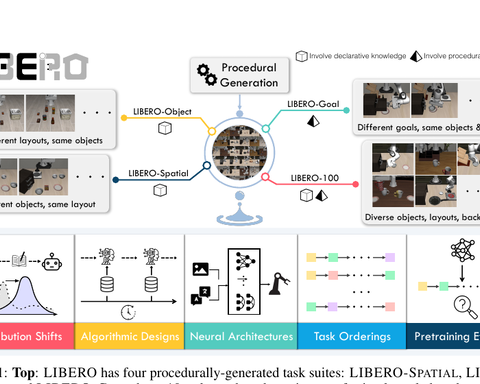
\includegraphics[width=1.803cm,height=1.402cm]{figures/img/collage_tiles/libero.png}}};
\draw[black!35,line width=0.35pt] (0.000,-1.280) rectangle (1.803,-2.682);
\node[anchor=north west,text=ACMDarkBlue,font=\tiny,inner sep=0] at (0.030,-2.702) {\href{https://arxiv.org/abs/2306.03310}{LIBERO}};
\node[anchor=north west,inner sep=0] at (1.873,-1.280) {\href{https://arxiv.org/abs/2112.03227}{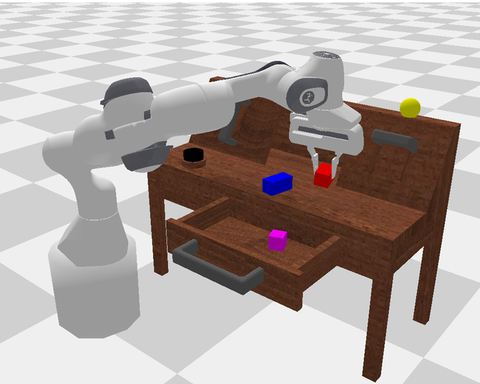
\includegraphics[width=1.803cm,height=1.402cm]{figures/img/collage_tiles/calvin.png}}};
\draw[black!35,line width=0.35pt] (1.873,-1.280) rectangle (3.676,-2.682);
\node[anchor=north west,text=ACMDarkBlue,font=\tiny,inner sep=0] at (1.903,-2.702) {\href{https://arxiv.org/abs/2112.03227}{CALVIN}};
\node[anchor=north west,inner sep=0] at (3.747,-1.280) {\href{https://arxiv.org/abs/1910.10897}{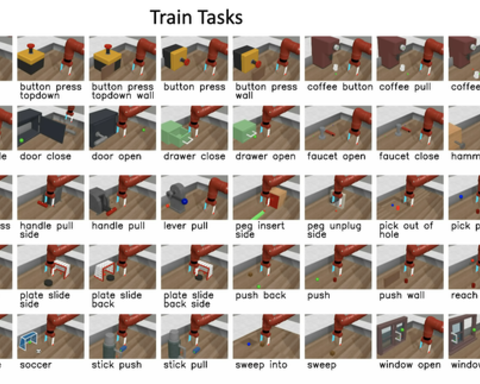
\includegraphics[width=1.803cm,height=1.402cm]{figures/img/collage_tiles/metaworld.png}}};
\draw[black!35,line width=0.35pt] (3.747,-1.280) rectangle (5.550,-2.682);
\node[anchor=north west,text=ACMDarkBlue,font=\tiny,inner sep=0] at (3.777,-2.702) {\href{https://arxiv.org/abs/1910.10897}{Meta-World}};
\node[anchor=north west,inner sep=0] at (0.000,-3.057) {\href{https://arxiv.org/abs/2302.04659}{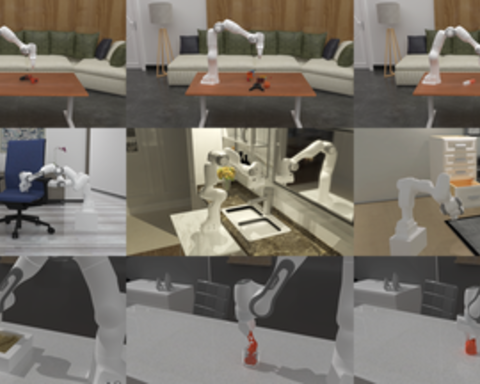
\includegraphics[width=1.803cm,height=1.402cm]{figures/img/collage_tiles/maniskill2.png}}};
\draw[black!35,line width=0.35pt] (0.000,-3.057) rectangle (1.803,-4.459);
\node[anchor=north west,text=ACMDarkBlue,font=\tiny,inner sep=0] at (0.030,-4.479) {\href{https://arxiv.org/abs/2302.04659}{ManiSkill2}};
\node[anchor=north west,inner sep=0] at (1.873,-3.057) {\href{https://arxiv.org/abs/2406.02523}{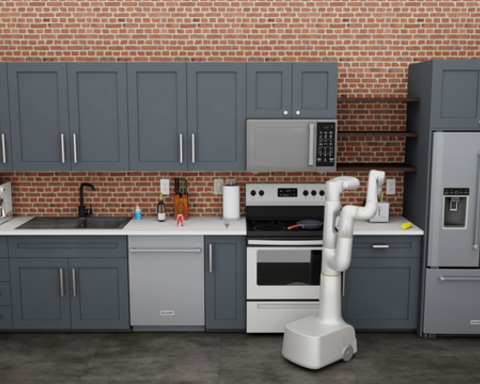
\includegraphics[width=1.803cm,height=1.402cm]{figures/img/collage_tiles/robocasa.png}}};
\draw[black!35,line width=0.35pt] (1.873,-3.057) rectangle (3.676,-4.459);
\node[anchor=north west,text=ACMDarkBlue,font=\tiny,inner sep=0] at (1.903,-4.479) {\href{https://arxiv.org/abs/2406.02523}{RoboCasa}};
\node[anchor=north west,inner sep=0] at (3.747,-3.057) {\href{https://arxiv.org/abs/2310.13724}{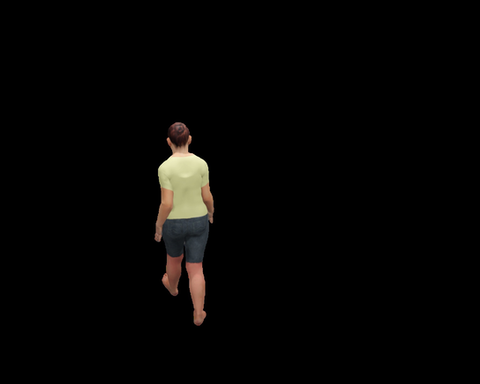
\includegraphics[width=1.803cm,height=1.402cm]{figures/img/collage_tiles/habitat30.png}}};
\draw[black!35,line width=0.35pt] (3.747,-3.057) rectangle (5.550,-4.459);
\node[anchor=north west,text=ACMDarkBlue,font=\tiny,inner sep=0] at (3.777,-4.479) {\href{https://arxiv.org/abs/2310.13724}{Habitat 3.0}};
\node[anchor=north west,inner sep=0] at (0.000,-4.833) {\href{https://arxiv.org/abs/1912.01734}{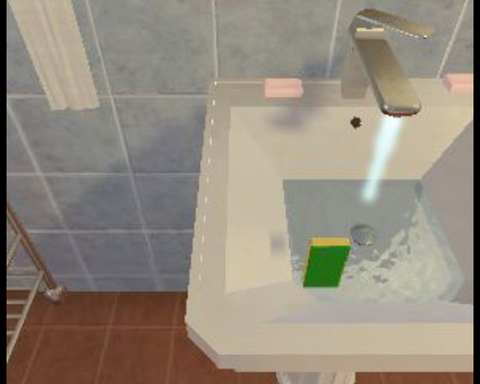
\includegraphics[width=1.803cm,height=1.402cm]{figures/img/collage_tiles/alfred.png}}};
\draw[black!35,line width=0.35pt] (0.000,-4.833) rectangle (1.803,-6.235);
\node[anchor=north west,text=ACMDarkBlue,font=\tiny,inner sep=0] at (0.030,-6.255) {\href{https://arxiv.org/abs/1912.01734}{ALFRED}};
\node[anchor=north west,inner sep=0] at (1.873,-4.833) {\href{https://arxiv.org/abs/2410.01345}{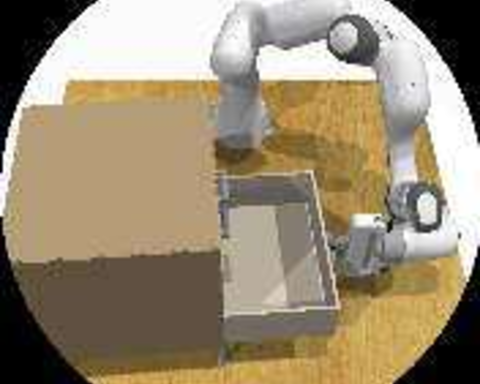
\includegraphics[width=1.803cm,height=1.402cm]{figures/img/collage_tiles/gembench.png}}};
\draw[black!35,line width=0.35pt] (1.873,-4.833) rectangle (3.676,-6.235);
\node[anchor=north west,text=ACMDarkBlue,font=\tiny,inner sep=0] at (1.903,-6.255) {\href{https://arxiv.org/abs/2410.01345}{GemBench}};
\node[anchor=north west,inner sep=0] at (3.747,-4.833) {\href{https://arxiv.org/abs/2412.18194}{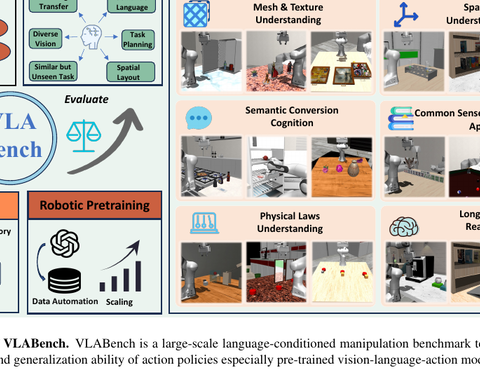
\includegraphics[width=1.803cm,height=1.402cm]{figures/img/collage_tiles/vlabench.png}}};
\draw[black!35,line width=0.35pt] (3.747,-4.833) rectangle (5.550,-6.235);
\node[anchor=north west,text=ACMDarkBlue,font=\tiny,inner sep=0] at (3.777,-6.255) {\href{https://arxiv.org/abs/2412.18194}{VLABench}};
\node[anchor=north west,inner sep=0] at (8.250,-1.280) {\href{https://arxiv.org/abs/2502.20694}{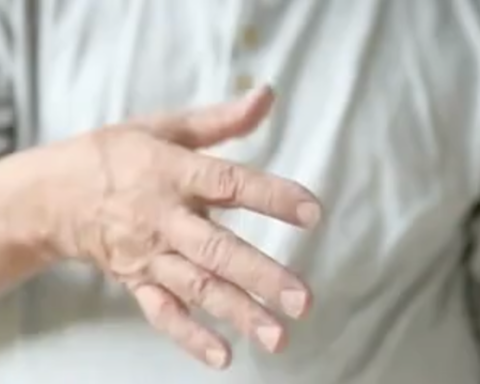
\includegraphics[width=1.803cm,height=1.402cm]{figures/img/collage_tiles/worldmodelbench.png}}};
\draw[black!35,line width=0.35pt] (8.250,-1.280) rectangle (10.053,-2.682);
\node[anchor=north west,text=ACMDarkBlue,font=\tiny,inner sep=0] at (8.280,-2.702) {\href{https://arxiv.org/abs/2502.20694}{WorldModelBench}};
\node[anchor=north west,inner sep=0] at (10.123,-1.280) {\href{https://arxiv.org/abs/2501.09038}{
\includegraphics[width=1.803cm,height=1.402cm]{figures/img/collage_tiles/physicsiq.png}}};
\draw[black!35,line width=0.35pt] (10.123,-1.280) rectangle (11.926,-2.682);
\node[anchor=north west,text=ACMDarkBlue,font=\tiny,inner sep=0] at (10.153,-2.702) {\href{https://arxiv.org/abs/2501.09038}{Physics-IQ}};
\node[anchor=north west,inner sep=0] at (11.997,-1.280) {\href{https://arxiv.org/abs/2504.00983}{
\includegraphics[width=1.803cm,height=1.402cm]{figures/img/collage_tiles/worldscore.png}}};
\draw[black!35,line width=0.35pt] (11.997,-1.280) rectangle (13.800,-2.682);
\node[anchor=north west,text=ACMDarkBlue,font=\tiny,inner sep=0] at (12.027,-2.702) {\href{https://arxiv.org/abs/2504.00983}{WorldScore}};
\node[anchor=north west,inner sep=0] at (8.250,-3.057) {\href{https://arxiv.org/abs/2505.09694}{
\includegraphics[width=1.803cm,height=1.402cm]{figures/img/collage_tiles/ewmbench.png}}};
\draw[black!35,line width=0.35pt] (8.250,-3.057) rectangle (10.053,-4.459);
\node[anchor=north west,text=ACMDarkBlue,font=\tiny,inner sep=0] at (8.280,-4.479) {\href{https://arxiv.org/abs/2505.09694}{EWMBench}};
\node[anchor=north west,inner sep=0] at (10.123,-3.057) {\href{https://arxiv.org/abs/2410.15461}{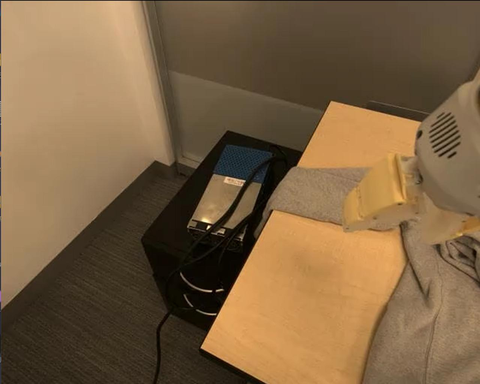
\includegraphics[width=1.803cm,height=1.402cm]{figures/img/collage_tiles/evabench.png}}};
\draw[black!35,line width=0.35pt] (10.123,-3.057) rectangle (11.926,-4.459);
\node[anchor=north west,text=ACMDarkBlue,font=\tiny,inner sep=0] at (10.153,-4.479) {\href{https://arxiv.org/abs/2410.15461}{EVA-Bench}};
\node[anchor=north west,inner sep=0] at (11.997,-3.057) {\href{https://arxiv.org/abs/2406.03520}{
\includegraphics[width=1.803cm,height=1.402cm]{figures/img/collage_tiles/videophy.png}}};
\draw[black!35,line width=0.35pt] (11.997,-3.057) rectangle (13.800,-4.459);
\node[anchor=north west,text=ACMDarkBlue,font=\tiny,inner sep=0] at (12.027,-4.479) {\href{https://arxiv.org/abs/2406.03520}{VideoPhy}};
\node[anchor=north west,inner sep=0] at (8.250,-4.833) {\href{https://arxiv.org/abs/2306.15668}{
\includegraphics[width=1.803cm,height=1.402cm]{figures/img/collage_tiles/physionpp.png}}};
\draw[black!35,line width=0.35pt] (8.250,-4.833) rectangle (10.053,-6.235);
\node[anchor=north west,text=ACMDarkBlue,font=\tiny,inner sep=0] at (8.280,-6.255) {\href{https://arxiv.org/abs/2306.15668}{Physion++}};
\node[anchor=north west,inner sep=0] at (10.123,-4.833) {\href{https://arxiv.org/abs/2106.08261}{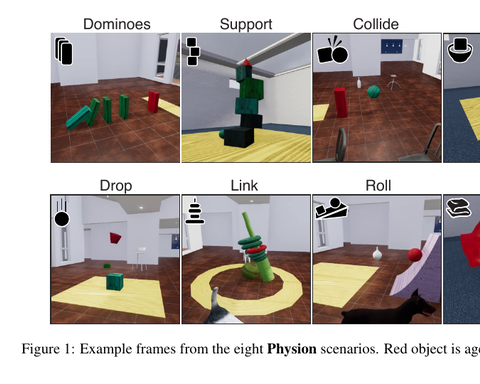
\includegraphics[width=1.803cm,height=1.402cm]{figures/img/collage_tiles/physion.png}}};
\draw[black!35,line width=0.35pt] (10.123,-4.833) rectangle (11.926,-6.235);
\node[anchor=north west,text=ACMDarkBlue,font=\tiny,inner sep=0] at (10.153,-6.255) {\href{https://arxiv.org/abs/2106.08261}{Physion}};
\node[anchor=north west,inner sep=0] at (11.997,-4.833) {\href{https://arxiv.org/abs/2310.11440}{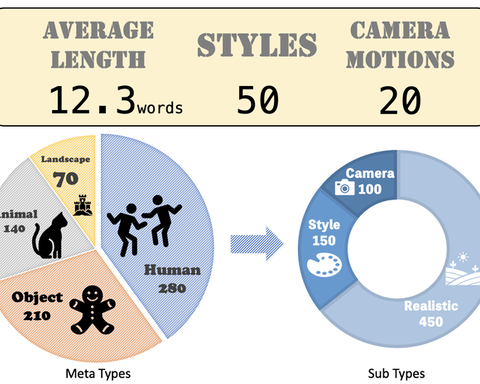
\includegraphics[width=1.803cm,height=1.402cm]{figures/img/collage_tiles/evalcrafter.png}}};
\draw[black!35,line width=0.35pt] (11.997,-4.833) rectangle (13.800,-6.235);
\node[anchor=north west,text=ACMDarkBlue,font=\tiny,inner sep=0] at (12.027,-6.255) {\href{https://arxiv.org/abs/2310.11440}{EvalCrafter}};
\end{tikzpicture}}
\caption{\textbf{Predict or Act?} The survey's organising question, posed with real benchmarks. \emph{Closed-loop} (left): policy and embodied suites score task success by running a policy in the environment. \emph{Open-loop} (right): world-model and video-generation benchmarks score prediction or generation quality with no action. The centre axis is the question neither pole answers, whether prediction earns a closed-loop advantage, built explicitly by only 11 of 160 benchmarks (Table~\ref{tab:landscape}). Every tile is a representative figure from the benchmark's paper and links to it; per-tile provenance is in Table~\ref{tab:collage_provenance}. Images \textcopyright\ their respective authors, reproduced for scholarly review.}
\Description{A two-pole collage of benchmark figures. A black title bar reads ``Predict or Act?''. The left band, CLOSED-LOOP, shows nine policy and embodied benchmark figures; the right band, OPEN-LOOP, shows nine world-model and video-generation benchmark figures; a centre spine contrasts task success (closed loop) with prediction quality (open loop) and notes that only 11 of 160 build the contrast.}
\label{fig:corpus_collage}
\end{figure*}


The gap is methodological rather than empirical. A world-model benchmark scores a rollout for
realism or physical plausibility and then stops; it never closes the loop, so it cannot report
whether the prediction would have helped a robot act. A task-success suite does close the loop, but
it hosts a single policy and is deliberately model-agnostic, so it never contrasts a world-model
policy against a direct VLA policy under one protocol. A benchmark that could answer the question
must run \emph{both} branches in one closed loop and report the per-capability gain
(Section~\ref{sec:gap}, Figure~\ref{fig:eval_loop}). Only a handful of recent
``bridge'' benchmarks attempt this, and none yet reports a capability-sliced VLA head-to-head.

This survey is therefore about \emph{evaluation}, not about models. It maps the benchmark landscape
that surrounds the question and asks which benchmarks could, in principle, establish an
advantage of prediction. We catalogue 160 web-verified benchmarks spanning 2017 to 2026 and organise
them by evaluation mode, robotic capability, and model family. The headline finding is stark: 138 of
the 160 benchmarks are model-agnostic and only 11 (7\%) build an explicit VLA-versus-world-model
contrast, counterfactual capability is almost entirely unmeasured, and only four benchmarks turn
prediction into executed action.

\paragraph{Contributions.} This survey offers the following.
\begin{itemize}
  \item An \textbf{operational taxonomy} of 160 robot-evaluation benchmarks across four evaluation
        lanes and twelve capability areas (Figure~\ref{fig:taxonomy_main}), with per-benchmark detail
        in Tables~\ref{tab:compare_main} and~\ref{tab:landscape} and placement rules in
        Table~\ref{tab:defs}.
  \item A \textbf{profile of the corpus} (Figures~\ref{fig:corpus_overview},
        \ref{fig:corpus_dist},~\ref{fig:lane_trend}) and two galleries of the benchmarks' own subject
        and results figures (Figures~\ref{fig:subject_gallery},~\ref{fig:results_gallery}), each panel
        provenance-tracked.
  \item A \textbf{coverage comparison} against the eight closest benchmark and evaluation surveys
        (Table~\ref{tab:survey_compare}): ours is the only one that crosses robotic capability with
        model family under a single protocol.
  \item A \textbf{contrast-gap analysis} (Section~\ref{sec:gap}): an evaluation loop that isolates
        the advantage of prediction (Figure~\ref{fig:eval_loop}), a disambiguation of the overloaded
        term ``world model'' (Table~\ref{tab:wm_senses}), and a lane-by-lane account of why the
        contrast is missing (Table~\ref{tab:branch_limits}).
  \item An \textbf{actionable protocol} for advantage-aware evaluation: four measurable quantities
        with named testbeds (Table~\ref{tab:future_metrics}, Figure~\ref{fig:future_protocol}).
\end{itemize}

\noindent The organising claim is deliberately modest. We do not argue that world models help, or
that they do not. We argue that the question is currently unanswerable with the benchmarks the field
has built, and we specify what a benchmark that could answer it would have to do.

\subsection{Related surveys and the empty cell}
\label{sec:related}

Table~\ref{tab:survey_compare} places the eight closest surveys and position papers against five axes
that a survey of predictive embodied evaluation could organise around: ($\alpha$) evaluation mode,
open- versus closed-loop, as the \emph{primary} axis; ($\beta$) robotic capability, such as
hidden-state, counterfactual, long-horizon, and social; ($\gamma$) a capability-by-model-family
cross-tabulation, direct VLA against latent, action-conditioned, and generative world models under
one protocol; ($\delta$) a behavioural advantage-of-prediction metric, which we \emph{assess} in the
literature rather than adopt; and ($\varepsilon$) a comprehensive benchmark catalogue. Existing
surveys populate $\varepsilon$ well and touch $\alpha$ and $\beta$ in passing, but the capability-by-family
cross-tab $\gamma$ is absent everywhere, and the advantage metric $\delta$ is reached only partially,
and only by a position paper~\cite{pos_yangyu}, never by a survey. Figure~\ref{fig:surveys} places
these works on a timeline: two predate the recent world-model wave, and the rest cluster in the last
two years, none of them crossing capability with family.

% Table 1 -- coverage of the closest benchmark/evaluation surveys vs. ours (the novelty gap).
% Marks transcribed from novelty_gap_B_benchmark.md and reconciled with a fresh parallel
% web-search audit (Yang Yu delta downgraded to partial; VLA-datasets venue = arXiv, not TMLR).
\begin{table}[t]
\centering
\footnotesize
\setlength{\tabcolsep}{4.5pt}
\renewcommand{\arraystretch}{1.25}
\resizebox{\textwidth}{!}{%
\begin{tabular}{@{}p{0.26\textwidth}c c *{5}{c}@{}}
\toprule
\textbf{Survey} & \textbf{Venue} & \textbf{Yr}
 & \shortstack{$\alpha$\\{\scriptsize mode}} & \shortstack{$\beta$\\{\scriptsize cap.}}
 & \shortstack{$\gamma$\\{\scriptsize family}} & \shortstack{$\delta$\\{\scriptsize metric}}
 & \shortstack{$\varepsilon$\\{\scriptsize catalog}}\\
\midrule
Evaluation of Embodied AI~\cite{survey_evalembodied} & Authorea & 2026 & \pp & \pp & \nn & \nn & \yy\\
VLA Datasets \& Bench.~\cite{survey_vladata} & arXiv & 2026 & \nn & \nn & \nn & \nn & \yy\\
Benchmark Construction~\cite{survey_benchconstruct} & arXiv & 2026 & \nn & \pp & \nn & \nn & \yy\\
RL Reproducibility~\cite{survey_rlrepro} & CoRL & 2020 & \nn & \nn & \nn & \nn & \nn\\
World Models for Robots~\cite{survey_wmrobot} & arXiv & 2026 & \pp & \nn & \pp & \pp & \pp\\
Embodied World Models~\cite{survey_embodiedwm} & preprint & 2026 & \pp & \nn & \pp & \nn & \pp\\
WM Evaluation \emph{(pos.)}~\cite{pos_yangyu} & arXiv & 2026 & \yy & \pp & \nn & \pp & \nn\\
Embodied AI: Simulators~\cite{survey_embodiedsim} & TETCI & 2022 & \pp & \pp & \nn & \nn & \yy\\
\midrule
\textbf{Ours (this survey)} & \dm & 2026 & \yy & \yy & \yy & \yy & \yy\\
\bottomrule
\end{tabular}}
\caption{\textbf{Topical coverage of the closest benchmark/evaluation surveys versus ours.}
\yy\ covered as an organising axis, \pp\ partial or mentioned in passing, \nn\ absent.
Axes: \textbf{$\alpha$} evaluation mode (open- vs closed-loop as the \emph{primary} axis);
\textbf{$\beta$} capability cuts (hidden-state, counterfactual, long-horizon, social);
\textbf{$\gamma$} capability~$\times$~model-family cross-tab (direct VLA vs latent /
action-conditioned / generative world models under one protocol); \textbf{$\delta$} behavioural
advantage-of-prediction metric (\emph{assessed, not adopted}; e.g.\ ACTION-ATLAS's World Advantage
Score); \textbf{$\varepsilon$} comprehensive benchmark catalogue. This survey is the only work that
covers \textbf{$\gamma$}, and \textbf{$\delta$} is otherwise reached only \emph{partially}, and only
by a \emph{position} paper~\cite{pos_yangyu}, never by a survey. Venues: CoRL, IEEE TETCI; the
remaining rows are arXiv or unrefereed preprints (Authorea, Preprints.org).}
\label{tab:survey_compare}
\end{table}

% Related benchmark/evaluation surveys as a horizontal timeline (dates web-verified).
% amber = refereed venue (CoRL, IEEE TETCI); blue = preprint; red star = ours.
% Marker labels are Name [cite] only (years live on the axis ticks), mirroring p1_fig3.
% Chronology: Lynnerup 2019, Duan 2021, then a 2026 cluster (Jan; Apr x3; Jun x2).
\begin{figure}[t]
\centering
\resizebox{\columnwidth}{!}{%
\begin{tikzpicture}[
 abv/.style={font=\scriptsize, anchor=south, align=center},
 blw/.style={font=\scriptsize, anchor=north, align=center},
 stem/.style={gray!55, line width=0.5pt},
]
 \draw[-{Stealth[length=3.2mm]}, line width=1.3pt, gray!65] (-0.4,0) -- (13.4,0);
 \node[font=\scriptsize\itshape, gray, anchor=west] at (13.0,-0.28) {time};
 % year ticks (compressed: a long gap, then the dense 2026 cluster)
 \foreach \x/\yr in {0.3/2019, 2.3/2021, 8.5/2026}{\draw[gray!35] (\x,-0.12)--(\x,0.12);
   \node[font=\footnotesize\bfseries,gray!80] at (\x,-1.15) {\yr};}
 \draw[gray!30,dashed] (3.3,-0.9)--(3.3,0.9); % break marker before the 2026 cluster
 % legend
 \filldraw[fill=secD,draw=hidden-draw] (-0.35,1.5) circle (3pt);
 \node[font=\scriptsize,gray,anchor=west] at (-0.12,1.5) {= refereed venue (CoRL, IEEE TETCI); others are preprints};
 % events (amber=refereed, blue=preprint); alternate above/below
 \filldraw[fill=secD,draw=hidden-draw] (0.3,0) circle (3.6pt);
 \draw[stem] (0.3,0.12)--(0.3,0.5); \node[abv] at (0.3,0.53) {\textbf{RL Reprod.}~\cite{survey_rlrepro}};
 \filldraw[fill=secD,draw=hidden-draw] (2.3,0) circle (3.6pt);
 \draw[stem] (2.3,-0.12)--(2.3,-0.5); \node[blw] at (2.3,-0.53) {\textbf{Embodied AI: Sim.}~\cite{survey_embodiedsim}};
 \filldraw[fill=secB,draw=hidden-draw] (5.0,0) circle (3.6pt);
 \draw[stem] (5.0,0.12)--(5.0,0.5); \node[abv] at (5.0,0.53) {\textbf{Eval.\ of Embodied AI}~\cite{survey_evalembodied}};
 \filldraw[fill=secB,draw=hidden-draw] (7.0,0) circle (3.6pt);
 \draw[stem] (7.0,-0.12)--(7.0,-0.5); \node[blw] at (7.0,-0.53) {\textbf{VLA Datasets}~\cite{survey_vladata}};
 \filldraw[fill=secB,draw=hidden-draw] (8.6,0) circle (3.6pt);
 \draw[stem] (8.6,0.12)--(8.6,0.5); \node[abv] at (8.6,0.53) {\textbf{WM for Robots}~\cite{survey_wmrobot}};
 \filldraw[fill=secB,draw=hidden-draw] (10.0,0) circle (3.6pt);
 \draw[stem] (10.0,-0.12)--(10.0,-0.5); \node[blw] at (10.0,-0.53) {\textbf{Embodied WM}~\cite{survey_embodiedwm}};
 \filldraw[fill=secB,draw=hidden-draw] (11.4,0) circle (3.6pt);
 \draw[stem] (11.4,0.12)--(11.4,0.5); \node[abv] at (11.4,0.53) {\textbf{Bench.\ Constr.}~\cite{survey_benchconstruct}};
 \filldraw[fill=secE!55,draw=hidden-draw] (12.5,0) circle (3.6pt);
 \draw[stem] (12.5,-0.12)--(12.5,-0.5); \node[blw] at (12.5,-0.53) {\textbf{WM Eval.} \emph{(pos.)}~\cite{pos_yangyu}};
 % Ours: bold red star endpoint
 \node[star,star points=5,star point ratio=2.4,fill=secE,draw=hidden-draw,minimum size=16pt,inner sep=0] at (13.1,0) {};
 \draw[secE!70!black,line width=0.6pt] (13.1,0.2)--(13.1,0.5);
 \node[abv,text=secE!45!black] at (13.1,0.6) {\textbf{Ours}};
\end{tikzpicture}}
\caption{The closest benchmark/evaluation surveys as a timeline. Two predate the recent wave, an
IEEE~TETCI survey of embodied-AI simulators and tasks~\cite{survey_embodiedsim} and a CoRL survey of
real-robot RL reproducibility~\cite{survey_rlrepro} (\textcolor{secD!55!black}{amber} = refereed
venue); the rest are 2026 preprints on embodied evaluation, VLA data, and world models. None
organises the robot-evaluation landscape by evaluation-mode $\times$ capability $\times$ model-family;
the sole work reaching the advantage-of-prediction axis is a \emph{position} paper~\cite{pos_yangyu}.
\textbf{Ours} ($\star$) fills that cell; per-axis coverage is in Table~\ref{tab:survey_compare}.}
\Description{A horizontal timeline of eight related surveys. Two amber refereed markers sit at 2019
(RL reproducibility, CoRL) and 2021 (embodied-AI simulators, IEEE TETCI); after a time break, a dense
cluster of 2026 preprint markers covers evaluation of embodied AI, VLA datasets, world models for
robots, embodied world models, benchmark construction, and a world-model-evaluation position paper. A
red star marks the present survey at the end.}
\label{fig:surveys}
\end{figure}

